\documentclass[12pt,compress,aspectratio=169]{beamer}

\mode<presentation>
{
  \usetheme{Singapore}
  \setbeamersize{text margin left=1cm,text margin right=1cm}
%  \setbeamertemplate{navigation symbols}{} % suppress nav bar
%  \setbeamercovered{transparent}
}
\usefonttheme{professionalfonts}
\usepackage{amsmath,bm}
\usepackage{siunitx}
%\usepackage{graphicx}
\usepackage{tikz}
\usepackage{mathpazo}
\usepackage[scaled]{helvet}
\usepackage{xcolor,colortbl}
%\usepackage{hyperref}

\usetikzlibrary{decorations.pathmorphing,patterns}

\sisetup{
  number-math-rm=\mathnormal,
  per-mode=symbol
}

\title{Simple Harmonic Motion}
\subtitle{Special AP/CAP Lecture}
\author[TML]{Dr.\ Timothy Leung}
\institute{Olympiads School}
\date{Fall 2019}

\newcommand{\pic}[2]{\includegraphics[width=#1\textwidth]{#2}}
\newcommand{\mb}[1]{\ensuremath\mathbf{#1}}
\newcommand{\eq}[2]{\vspace{#1}{\Large\begin{displaymath}#2\end{displaymath}}}

\begin{document}

\begin{frame}
  \maketitle
\end{frame}


\section{Hooke's Law}

\begin{frame}{Hooke's Law}
  Hooke's law for an ideal spring relates the force exerted by a compressed (or
  stretched) spring onto another object (\textbf{spring force} $\mb{F}_s$) to
  the stiffness of the spring (\textbf{spring constant} $k$) and spring
  displacement $\mb{x}$:

  \eq{-.2in}{
    \boxed{\mb{F}_s=-k\mb{x}}
  }
  \begin{center}
    \begin{tabular}{l|c|c}
      \rowcolor{pink}
      \textbf{Quantity} & \textbf{Symbol} & \textbf{SI Unit} \\ \hline
      Spring force                    & $\mb{F}_s$ & \si{\newton}\\
      Spring constant                 & $k$ & \si{\newton\per\metre}\\
      Amount of extension/compression & $\mb{x}$ & \si{\metre}
    \end{tabular}
  \end{center}
  Spring constant is also called \textbf{Hooke's constant} or
  \textbf{force constant}.
\end{frame}



\begin{frame}{Elastic Potential Energy}
  Applying Hooke's law in the work equation gives the amount of 
  \textbf{elastic potential energy} stored in the spring when it is
  compressed or stretched:

  \eq{-.25in}{
    W=\int^{x_2}_{x_1}\mb{F}_e\cdot d\mb{x}=-\int^{x_2}_{x_1}kxdx
    =-\frac{1}{2}kx^2\Big|^{x_2}_{x_1}=-\Delta U_e
  }

  where elastic potential energy is defined as

  \eq{-.2in}{
    \boxed{U_e=\frac{1}{2}kx^2}
  }
\end{frame}



\section{Spring-Mass}

\begin{frame}{Mass on a Spring}
  Consider the forces acting on a mass connected horizontally to a spring

  \begin{center}
    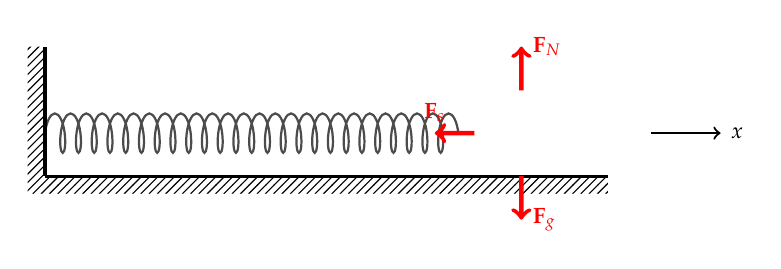
\begin{tikzpicture}[scale=1.1]
      \node[fill=blue!70,inner sep=4.5mm,white] (a) at (5.5,1) {$m$};
      \draw[thick,draw=black!70,
        decoration={aspect=0.3,segment length=2mm, amplitude=2.5mm, coil},
        decorate] (0,1)--(4.95,1);
      \fill [pattern=north east lines] (6.5,0.5)--(6.5,0.3)--(-0.2,0.3)
      --(-0.2,2)--(0,2)--(0,0.5)--cycle;
      \draw[very thick] (0,0.5)--(6.5,0.5);
      \draw[very thick] (0,0.5)--(0,2);
      \draw[ultra thick,->,red](a)--(5.5,0)
      node[pos=1,right]{\footnotesize $\mb{F}_g$};
      \draw[ultra thick,->,red](a)--(5.5,2)
      node[pos=1,right]{\footnotesize $\mb{F}_N$};
      \draw[ultra thick,->,red](a)--(4.5,1)
      node[pos=1,above]{\footnotesize $\mb{F}_s$};
      \draw[->,thick](7,1)--(7.8,1) node[pos=1,right]{\footnotesize $x$};
    \end{tikzpicture}
  \end{center}
  $\mb{F}_g$ and $\mb{F}_N$ cancel out, so net force is due only to spring
  force $\mb{F}_s=-k\mb{x}$. This is true both when the spring is in
  compression or extension. (In the diagram above, the spring is in extension.)
\end{frame}

\begin{frame}{Mass on a Spring}
  Applying Newton's 2nd law in the $x$-direction:

  \eq{-.25in}{
    \sum F=F_s=ma\quad\longrightarrow\quad-kx=m\frac{d^2x}{dt^2}
  }

  The equation above is generally written in the standard form

  \eq{-.15in}{
    \boxed{\frac{d^2x}{dt^2}+\frac{k}{m}x=0}
  }
  
  This equation is called a
  \emph{second-order ordinary differential equation with constant coefficients}.
\end{frame}



\begin{frame}{Mass on a Spring}
  
  \eq{-.01in}{
    \boxed{\frac{d^2x}{dt^2}+\frac{k}{m}x=0}
  }
  \begin{itemize}
  \item To solve the above equation, we look for a function $x(t)$ where the
    second derivative $x''(t)$ looks like $x(t)$ itself but with a negative sign
  \item The obvious choice are the two trigonometric functions: $\sin(t)$ and
    $\cos(t)$
  \item<2-> We start with this general form
    
    \eq{-.3in}{
      x(t)=A\sin(\omega t+\phi)
    }
%    
%    \vspace{-.2in}We usually prefer using $\sin$ over $\cos$, but the two
%    functions only differ in $\phi$
  \end{itemize}
\end{frame}


\begin{frame}{Mass on a Spring}

  \eq{-.01in}{
    \boxed{\frac{d^2x}{dt^2}+\frac{k}{m}x=0}
  }
  
  Starting with the general form, we can take the time derivatives to obtain
  the velocity and acceleration of the mass as a function of time:
 
  \vspace{-.35in}{\Large
    \begin{align*}
      x(t)&=A\sin(\omega t+\phi)\\
      v(t)&=A\omega\cos(\omega t+\phi)\\
      a(t)&=-A\omega^2\sin(\omega t+\phi)=-\omega^2x
    \end{align*}
  }
  
  \vspace{-.2in}where $\omega$ is the angular frequency, and $A$ is the
  amplitude of the oscillation and $\phi$ is a phase shift that depends on the
  initial condition
\end{frame}



\begin{frame}{Mass on a Spring}{Angular Frequency}
  Substituting expressions of $x(t)$ and $a(t)=x''(t)$ into the ODE, we find
  that the solution is satisfied if angular frequency is related to the spring
  constant and mass by:

  \eq{-.2in}{
    \boxed{\omega=\sqrt{\frac{k}{m}}}
  }

  The angular frequency for the undamped oscillator is called the
  \textbf{natural frequency}.
\end{frame}



\begin{frame}{Mass on a Spring}{Frequency and Period}
  The period $T$ and frequency $f$ of the motion are given by:

  \eq{-.2in}{
    \boxed{f=\frac{\omega}{2\pi}=\frac{1}{2\pi}\sqrt{\frac{k}{m}}}\quad\quad
    \boxed{T=\frac{1}{f}=2\pi\sqrt{\frac{m}{k}}}
  }
  Angular frequency, frequency and period do not depend on amplitude $A$
\end{frame}



\begin{frame}{Mass on a Spring}{Side Note \#1}
  \textbf{Side Note \#1:} The solution to any ODE is the linear combination of
  \emph{all} possible solutions, i.e.:

  \eq{-.2in}{
    x(t)=c_1\sin(\omega t)+c_2\cos(\omega t)
  }

  Where $c_1$ and $c_2$ are constant coefficients based on the initial
  conditions. The solution form that was shown in previous slides are in fact
  identical to this solution.
\end{frame}



\begin{frame}{Mass on a Spring}{Side Note \#2}
  \textbf{Side Note \#2:} When searching for a solution to the ODE, one may
  ``guess'' a solution that is the exponential function, where its derivatives
  have the same form as the function itself, i.e.:

  \eq{-.3in}{
       x(t)=e^{\omega t}
  }

  \vspace{-.15in}However, the second derivative of $e^{\omega t}$ does not have
  the negative sign that is needed. But if the exponential function is
  complex:

  \eq{-.25in}{
    x(t)=e^{i\omega t}
  }

  \vspace{-.15in}then the 2nd derivative \emph{will} in fact have the negative
  sign:

  \eq{-.25in}{
    x'(t)=i\omega e^{i\omega t}\quad\rightarrow\quad
    x''(t)=i^2\omega^2 e^{i\omega t}=-\omega^2 e^{i\omega t}
  }
\end{frame}



\begin{frame}{Mass on a Spring}{Side Note \#2}
  This should not come as a surprise, since the complex exponential function
  and the sinusoidal functions are related:

  \eq{-.2in}{
    e^{it}=\sin(t)+i\cos(t)
  }
\end{frame}

\begin{frame}{Vertical Spring-Mass System}
  \begin{columns}
    \column{.17\textwidth}
    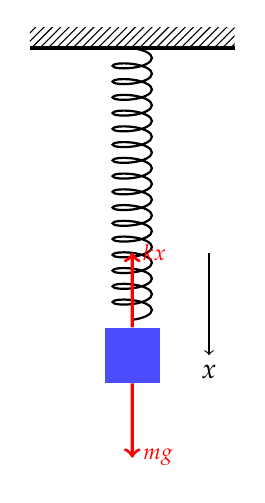
\begin{tikzpicture}[scale=1.3]
      \node[fill=blue!70,inner sep=3.5mm] (b) at (1,2) {};
      \draw[thick,
        decoration={aspect=0.3,segment length=2mm, amplitude=2.5mm, coil},
        decorate] (1,5)--(b); 
      \fill [pattern=north east lines] (0,5) rectangle (2,5.2);
      \draw[ultra thick] (0,5)--(2,5);
      \draw[->](1.75,3)--(1.75,2) node[pos=1,below]{$x$};
      \draw[very thick,->,red](b)--(1,1) node[pos=1,right]{\footnotesize $mg$};
      \draw[very thick,->,red](b)--(1,3) node[pos=1,right]{\footnotesize $kx$};
    \end{tikzpicture}

    \column{.85\textwidth}
    For a vertical spring-mass system, the analysis is \emph{slightly} more
    complicated (we have to consider weight as well):

    \eq{-.2in}{
      mg-kx=m\frac{d^2x}{dt^2}
    }

    \vspace{-.15in}But since $mg$ is a constant, the only difference is the
    addition of a constant $B$ in our expression of $x(t)$:
    
    \vspace{-.4in}{\Large
      \begin{align*}
        x(t)&=A\sin(\omega t+\phi) +B\\
        v(t)&=A\omega\cos(\omega t+\phi)\\
        a(t)&=-A\omega^2\sin(\omega t+\phi)
      \end{align*}
    }
  \end{columns}
\end{frame}



\begin{frame}{Vertical Spring-Mass System}
  \begin{columns}
    \column{.17\textwidth}
    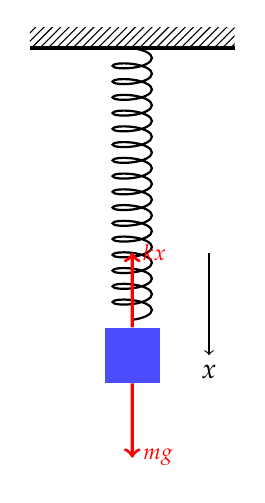
\begin{tikzpicture}[scale=1.3]
      \node[fill=blue!70,inner sep=3.5mm] (b) at (1,2) {};
      \draw[thick,
        decoration={aspect=0.3,segment length=2mm, amplitude=2.5mm, coil},
        decorate] (1,5)--(b); 
      \fill [pattern=north east lines] (0,5) rectangle (2,5.2);
      \draw[ultra thick] (0,5)--(2,5);
      \draw[->](1.75,3)--(1.75,2) node[pos=1,below]{$x$};
      \draw[very thick,->,red](b)--(1,1) node[pos=1,right]{\footnotesize $mg$};
      \draw[very thick,->,red](b)--(1,3) node[pos=1,right]{\footnotesize $kx$};
    \end{tikzpicture}

    \column{.85\textwidth}
    Substituting $x(t)$ and $x''(t)$ into the differential equation gives

    \eq{-.2in}{
      B=\frac{mg}{k}
    }

    which is just the stretching of the spring due to its weight

    \vspace{.2in}Angular frequency is the same as the horizontal case:

    \eq{-.2in}{
      \omega=\sqrt{\frac{k}{m}}
    }
  \end{columns}
\end{frame}



\begin{frame}{Conservation of Energy in a Spring-Mass System}

  In the spring-mass systems, if there are no frictional losses, then the only
  forces doing work are the spring force (horizontal and vertical) and gravity
  (vertical). Both forces are \emph{conservative}, therefore the total
  mechanical energy is conserved:

  \eq{-.2in}{
    K_1 + U_{e,1} + U_{g,1} = K_2 + U_{e,2} + U_{g,2}
  }
  
  For the horizontal spring-mass system, the total energy is:
    
  \eq{-.2in}{
    E_T=\frac{1}{2}kA^2
  }
\end{frame}


%\begin{frame}{Simple Example}
%  \textbf{Example 2:} A mass suspended from a spring is oscillating up and
%  down. Consider the following two statements:
%  \begin{enumerate}
%  \item At some point during the oscillation, the mass has zero velocity but it
%    is accelerating
%  \item At some point during the oscillation, the mass has zero velocity and
%    zero acceleration.
%  \end{enumerate}
%
%  \begin{enumerate}[(a)]
%  \item Both occur at some time during the oscillation
%  \item Neither occurs during the oscillation
%  \item Only (1) occurs
%  \item Only (2) occurs
%  \end{enumerate}
%\end{frame}
%
%
%
%\begin{frame}{Another Example}
%  \textbf{Example 3:} An object of mass \SI{5}{\kg} hangs from a spring and
%  oscillates with a period of \SI{0.5}{\second}. By how much will the
%  equilibrium length of the spring be shortened when the object is removed.
%  \begin{enumerate}[(a)]
%  \item\SI{0.75}{\centi\metre}
%  \item\SI{1.50}{\centi\metre}
%  \item\SI{3.13}{\centi\metre}
%  \item\SI{6.20}{\centi\metre}
%  \end{enumerate}
%\end{frame}



\section{Simple Pendulum}

\begin{frame}{What About a Pendulum?}
  \begin{columns}
    \column{.75\textwidth}
    \begin{itemize}
    \item Pendulums also exhibit oscillatory motion
    \item For a pendulum, there are two forces acting on the mass: weight
      $F_g=mg$ and tension $T$
    \item When the mass is deflected by an angle $\theta$, it's easy to show
      (using polar coordinates) that the force in the angular direction is
      $F_\theta=-mg\sin\theta$
    \item We needn't worry about the radial direction because it doesn't
      have anything to do with the restoring force
    \end{itemize}

    \column{.25\textwidth}
    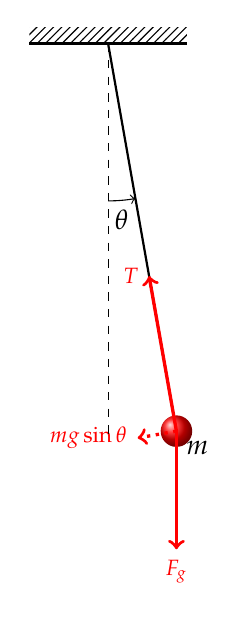
\begin{tikzpicture}
      \fill[pattern=north east lines] (-1,0) rectangle (1,0.2);
      \draw[very thick](-1,0)--(1,0);
      \begin{scope}[rotate=10]
        \draw[thick](0,0)--(0,-5);
        \tikzstyle{balloon}=[ball color=red];    
        \shade[balloon] (0,-5) circle (0.2) node[below right]{$m$};
        \draw[dotted,->,very thick,red](0,-5)--(-0.5,-5)
        node[pos=1,left]{\footnotesize $mg\sin\theta$};
        \draw[->,very thick,red](0,-5)--(0,-3)
        node[pos=1,left]{\footnotesize $T$};
        \draw[->,very thick,red, rotate around={-10:(0,-5)}](0,-5)--(0,-6.5)
        node[pos=1,below]{\footnotesize $F_g$};
      \end{scope}
      \draw[dashed,thin](0,0)--(0,-5);
      \draw[->](0,-2) arc(270:280:2) node[pos=0.5,below]{$\theta$};
    \end{tikzpicture}
  \end{columns}
\end{frame}



\begin{frame}{The Pendulum}
  \begin{columns}
    \column{0.75\textwidth}
    Substitute $F_\theta$ into Newton's second law, and cancelling mass term, we
    get:

    \eq{-.45in}{
      F_\theta=ma_\theta\quad\longrightarrow\quad
      -g\sin\theta=L\frac{d^2\theta}{dt^2}
    }

    For small angles, $\sin\theta\approx\theta$, and we get the ODE for the
    pendulum:
      
    \eq{-.25in}{
      \frac{d^2\theta}{dt^2}+\frac{g}{L}\theta=0
    }
    
    This ODE has the same form as the spring-mass system!
    
    \column{.25\textwidth}
    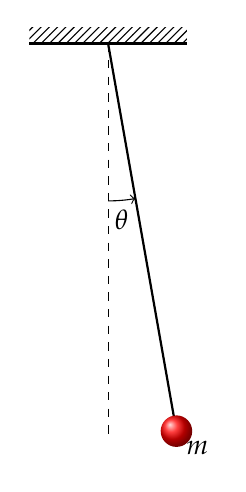
\begin{tikzpicture}
      \fill[pattern=north east lines] (-1,0) rectangle (1,0.2);
      \draw[very thick](-1,0)--(1,0);
      \begin{scope}[rotate=10]
        \draw[thick](0,0)--(0,-5);
        \tikzstyle{balloon}=[ball color=red];    
        \shade[balloon] (0,-5) circle (0.2) node[below right]{$m$};
      \end{scope}
      \draw[dashed,thin](0,0)--(0,-5);
      \draw[->](0,-2) arc(270:280:2) node[pos=0.5,below]{$\theta$};
    \end{tikzpicture}
  \end{columns}
\end{frame}


\begin{frame}{Ordinary Differential Equation for the Pendulum}
  \begin{itemize}
  \item The solution for $\theta(t)$ is very similar to the spring-mass system:

    \eq{-.25in}{
      \boxed{\theta(t)=\theta_\mathrm{max}\sin(\omega t+\phi)}
    }

    \vspace{-.15in}where $\omega$ is given by
    
    \eq{-.15in}{
      \boxed{\omega=\sqrt{\frac{g}{L}}}
    }

    \vspace{-.1in} and $\phi$ is a phase shift based on the initial condition
    of the pendulum.
  \item Remember that this equation is only valid for small angles, i.e.\
    $\theta_\mathrm{max}<\ang{15}$
  \end{itemize}
\end{frame}



%\begin{frame}{Pendulum Example Problem}
%  \textbf{Example 4:} A simple pendulum consists of a mass $m$ attached to a
%  light string of length $l$. If the system is oscillating through small
%  angles, which of the following is true
%  \begin{enumerate}[(a)]
%  \item The frequency is independent of the acceleration due to gravity, $g$.
%  \item The period depends on the amplitude of the oscillation.
%  \item The period is independent of the mass $m$.
%  \item The period is independent of the length $l$.
%  \end{enumerate}
%\end{frame}



\begin{frame}{A Pendulum Example}
  \textbf{Example:} A bucket full of water is attached to a rope and allowed
  to swing back and forth as a pendulum from a fixed support. The bucket has a
  hole in its bottom that allows water to leak out. How does the period of
  motion change with the loss of water?
  \begin{enumerate}[(a)]
  \item The period does not change.
  \item The period continuously decreases.
  \item The period continuously increases.
  \item The period increases to some maximum and then decreases again.
  \end{enumerate}
\end{frame}


\begin{frame}{Think About $g$}
  \textbf{Example:} A little girl is playing with a toy pendulum while riding
  in an elevator. Being an astute and educated young lass, she notes that the 
  period of the pendulum is $T=\SI{.5}{\second}$. Suddenly the cables
  supporting the elevator break and all  of the brakes and safety features fail
  simultaneously. The elevator plunges into free fall. The young girl is
  astonished to discover that the pendulum has:
  \begin{enumerate}[(a)]
  \item continued oscillating with a period of \SI{.5}{\second}.
  \item stopped oscillating entirely.
  \item decreased its rate of oscillation to have a longer period.
  \item increased its rate of oscillation to have a lesser period.
  \end{enumerate}
\end{frame}



\section{Damped Oscillation}

\begin{frame}{It's Never Perfect}
  In reality, there are friction, or drag, or other damping forces present in
  the spring-mass system, represented schematically like the shock absorber:
  \begin{center}
    \vspace{-.15in}
    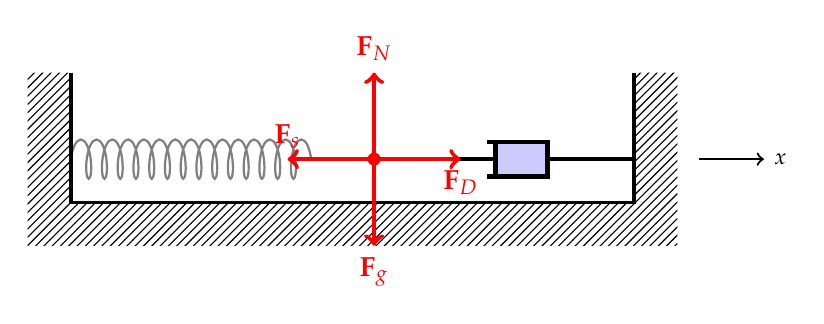
\begin{tikzpicture}[scale=1.1]
      \node[fill=blue!40!white,inner sep=4.5mm,white] (a) at (3.5,1) {$m$};
      \draw[thick,draw=black!50,
        decoration={aspect=0.3,segment length=2mm, amplitude=2.5mm, coil},
        decorate] (0,1)--(2.95,1);
      \fill[pattern=north east lines](-.5,2)--(-.5,0)--(7,0)--(7,2)--(6.5,2)
      --(6.5,.5)--(0,.5)--(0,2)--cycle;
      \draw[very thick] (0,2)--(0,.5)--(6.5,.5)--(6.5,2);
      \draw[->,thick](7.25,1)--(8,1) node[pos=1,right]{\footnotesize $x$};
      \uncover<2->{
        \draw[fill=blue!20!white] (4.9,.8) rectangle(5.5,1.2);
        \draw[ultra thick](4.05,1)--(4.9,1);
        \draw[ultra thick](4.9,.8)--(4.9,1.2);
        \draw[ultra thick](4.8,1.2)--(5.5,1.2)--(5.5,.8)--(4.8,.8);
        \draw[ultra thick](5.5,1)--(6.5,1);
      }
      \uncover<3->{
        \fill[red] (3.5,1)circle(.075);
        \draw[ultra thick,->,red](3.5,1)--(3.5,0) node[pos=1,below]{$\mb{F}_g$};
        \draw[ultra thick,->,red](3.5,1)--(3.5,2) node[pos=1,above]{$\mb{F}_N$};
        \draw[ultra thick,->,red](3.5,1)--(2.5,1) node[pos=1,above]{$\mb{F}_s$};
        \draw[ultra thick,->,red](3.5,1)--(4.5,1) node[pos=1,below]{$\mb{F}_D$};
      }
    \end{tikzpicture}
  \end{center}
  \uncover<4->{
    \vspace{-.15in}The damping force is typically related to velocity, in the
    opposite direction:

    \eq{-.3in}{
      \mb{F}_D=-b\mb{v}^n
    }

    \vspace{-.2in}In the simplest case is to use $n=1$ to represent viscous
    effects.
  }
\end{frame}



\begin{frame}{Damped Oscillator}
%  \begin{center}
%    \begin{tikzpicture}[scale=.8]
%      \node[fill=blue!40!white,inner sep=3mm,white] (a) at (3.5,1) {$m$};
%      \draw[thick,draw=black!50,
%        decoration={aspect=0.3,segment length=2mm, amplitude=2.5mm, coil},
%        decorate] (0,1)--(2.95,1);
%      \fill[pattern=north east lines](-.5,2)--(-.5,0)--(7,0)--(7,2)--(6.5,2)
%      --(6.5,.5)--(0,.5)--(0,2)--cycle;
%      \draw[very thick] (0,2)--(0,.5)--(6.5,.5)--(6.5,2);
%      \draw[fill=blue!20!white] (4.9,.8) rectangle(5.5,1.2);
%      \draw[ultra thick](4.05,1)--(4.9,1);
%      \draw[ultra thick](4.9,.8)--(4.9,1.2);
%      \draw[ultra thick](4.8,1.2)--(5.5,1.2)--(5.5,.8)--(4.8,.8);
%      \draw[ultra thick](5.5,1)--(6.5,1);
%      \fill[red] (3.5,1)circle(.075);
%      \draw[ultra thick,->,red](3.5,1)--(3.5,0) node[pos=1,below]{$\mb{F}_g$};
%      \draw[ultra thick,->,red](3.5,1)--(3.5,2) node[pos=1,above]{$\mb{F}_N$};
%      \draw[ultra thick,->,red](3.5,1)--(2.5,1) node[pos=1,above]{$\mb{F}_s$};
%      \draw[ultra thick,->,red](3.5,1)--(4.5,1) node[pos=1,below]{$\mb{F}_D$};
%    \end{tikzpicture}
%  \end{center}
%  \vspace{-.15in}
  The 2nd-order ODE is obtained by applying Newton's second law of motion:

  \eq{-.25in}{
    \sum F=F_s+F_D=ma\quad\rightarrow\quad -kx-b\frac{dx}{dt}=\frac{d^2x}{dt^2}
  }

  Arranging into standard form:
  
  \eq{-.15in}{
    \boxed{\frac{d^2x}{dt^2}+\frac{b}{m}\frac{dx}{dt}+\frac{k}{m}x=0}
  }

  The solution to this ODE is still relatively straightforward.
\end{frame}



\begin{frame}{Damped Oscillator}
  The solution to the damped oscillator is a standard problem in calculus
  class. It is the product of a exponential decay and a sinusoidal function:

  \eq{-.2in}{
    x(t)=A_0e^{-\frac{b}{2m}t}\sin(\omega't+\phi)
  }

  \vspace{-.15in}where $A_0$ is the initial amplitude of the damped oscillator,
  and the angular frequency is now given by:

  \eq{-.2in}{
    \boxed{
      \omega'=\sqrt{\omega_0^2-\left(\frac{b}{2m}\right)^2}
      \quad{\text{where}}\quad
      \omega_0=\sqrt{\frac{k}{m}}
    }
  }
  
  \vspace{-.15in}The angular frequency $\omega'$ of the damped oscillator
  differs from the undamped case $\omega_0$ depending on the damping factor
  $b$.
\end{frame}


\begin{frame}{Critical Damping}
  \textbf{Critical damping} occurs when the angular frequency $\omega'$ term
  is zero:
  
  \eq{-.2in}{
    \omega'=\sqrt{\omega_0^2-\left(\frac{b}{2m}\right)^2}=0
  }

  which occurs when the damping constant is:

  \eq{-.2in}{
    \boxed{b_{\textrm{critical}}=2m\omega_0}
  }
  \begin{itemize}
  \item A critically damped system returns to its equilibrium position in the
    shortest time with \emph{no} oscillation
  \item When $b>b_{\textrm{critical}}$, the system is \textbf{over-damped}
  \item Critical or near-critical damping is desired in many engineering designs
      \begin{itemize}
      \item Example: shock absorbers on car suspensions
      \end{itemize}
  \end{itemize}
\end{frame}



\begin{frame}{Comparing Damped System}
  \begin{center}
    \pic{.5}{oscda8.png}
  \end{center}
  The motion of the damped oscillator is not strictly periodic.
\end{frame}


\begin{frame}{Energy in a Damped System}
  The damping force (non-conservative) dissipates energy from the oscillator at
  a rate of:

  \eq{-.3in}{
    P=\frac{dE}{dt}=\mb{F}_D\cdot\mb{v}=-bv^2
  }

  \vspace{-.1in}As velocity relate to energy by: $(v_{\textrm{av}})^2=E/m$, power
  dissipation is a first-order linear ODE:

  \eq{-.25in}{
    \frac{dE}{dt}=-\frac{b}{m}E
  }

  The solution to the ODE shows the total amount of energy as a
  function of time:

  \eq{-.2in}{
    \boxed{E(t)=E_0e^{-\frac{b}{m}t}=E_0e^{-\frac{t}{\tau}}}
    }
\end{frame}



\section{Driven Oscillation}

\begin{frame}{Forced Harmonic Motion}
  To keep a damped system going, energy must be added into the system. Assuming
  that the system is subjected to an external force that is harmonic with time:

  \eq{-.2in}{
    F_{\textrm{ext}}=F_0\sin(\omega t)
  }
  \begin{center}
    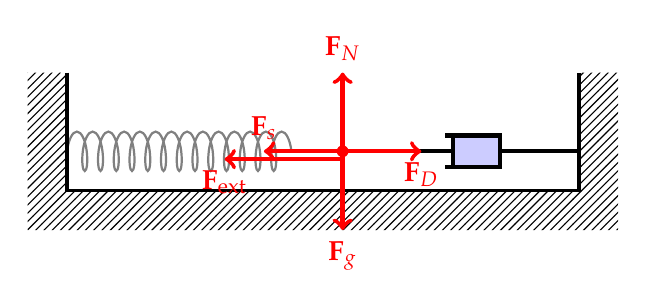
\begin{tikzpicture}
      \node[fill=blue!40!white,inner sep=3.5mm,white] (a) at (3.5,1) {$m$};
      \draw[thick,draw=black!50,
        decoration={aspect=0.3,segment length=2mm, amplitude=2.5mm, coil},
        decorate] (0,1)--(2.95,1);
      \fill[pattern=north east lines](-.5,2)--(-.5,0)--(7,0)--(7,2)--(6.5,2)
      --(6.5,.5)--(0,.5)--(0,2)--cycle;
      \draw[very thick] (0,2)--(0,.5)--(6.5,.5)--(6.5,2);
      \draw[fill=blue!20!white] (4.9,.8) rectangle(5.5,1.2);
      \draw[ultra thick](4.05,1)--(4.9,1);
      \draw[ultra thick](4.9,.8)--(4.9,1.2);
      \draw[ultra thick](4.8,1.2)--(5.5,1.2)--(5.5,.8)--(4.8,.8);
      \draw[ultra thick](5.5,1)--(6.5,1);
      \fill[red] (3.5,1)circle(.075);
      \draw[ultra thick,->,red](3.5,1)--(3.5,0) node[pos=1,below]{$\mb{F}_g$};
      \draw[ultra thick,->,red](3.5,1)--(3.5,2) node[pos=1,above]{$\mb{F}_N$};
      \draw[ultra thick,->,red](3.5,1)--(2.5,1) node[pos=1,above]{$\mb{F}_s$};
      \draw[ultra thick,->,red](3.5,.9)--(2,.9)
      node[pos=1,below]{$\mb{F}_{\textrm{ext}}$};
      \draw[ultra thick,->,red](3.5,1)--(4.5,1) node[pos=1,below]{$\mb{F}_D$};
    \end{tikzpicture}
  \end{center}
\end{frame}



\begin{frame}{Forced Harmonic Motion}
  Again, the second-order ordinary differential equation is obtained by
  applying Newton's second law of motion:
  
  \eq{-.2in}{
    \sum F=-kx-bv+F_0\sin(\omega t)=ma
  }

  Rearranging the terms gives a similar ODE to the damped case, but with the
  additional external force term on the right-hand side:

  \eq{-.2in}{
    \boxed{m\frac{d^2x}{dt^2}+b\frac{dx}{dt}+kx=F_0\sin(\omega t)}
  }

\end{frame}



\begin{frame}{Forced Harmonic Motion}
  \eq{-.02in}{
    \boxed{m\frac{d^2x}{dt^2}+b\frac{dx}{dt}+kx=F_0\sin(\omega t)}
  }
  
  The solution to this ODE has two components:
  \begin{itemize}
  \item A \textbf{transient solution} that is identical to that of the damped
    oscillator
    \begin{itemize}
    \item Obtained by setting the external force term to zero
    \item Depends on the initial condition
    \item Solution becomes negligible over time because of exponential-decay
    \end{itemize}
  \item A \textbf{steady-state solution} which does not depend on the initial
    condition
  \end{itemize}
\end{frame}



\begin{frame}{Forced Harmonic Motion}
  Solving for the steady-state solution will be left as a (straightforward but
  not simple) exercise in calculus, but it can be shown that the solution is a
  harmonic motion at the frequency $\omega$ of the external force:

  \eq{-.2in}{
    \boxed{x(t)=A\sin(\omega t+\phi)}
  }
  
  \vspace{-.1in}where the amplitude of the oscillation $A$ and phase constant
  $\phi$ are given by:

  \eq{-.3in}{
    \boxed{A=\frac{F_0}{\sqrt{m^2(\omega_0^2-\omega^2)^2+b^2\omega^2}}}
    \quad\;\;
    \boxed{\tan\phi=\frac{b\omega}{m(\omega_0^2-\omega^2)}}
  }
\end{frame}



\begin{frame}{Resonance}
  \textbf{Resonance} is caused by in-phase excitation at natural frequency.
  This means that:
  \begin{itemize}
  \item The frequency of the driving force is same as the natural frequency of
    the oscillator

    \eq{-.2in}{
      \omega=\omega_0\quad\text{where}\quad\omega_0=\sqrt{\frac{k}{m}}
    }
  \item The driving force follows the motion of the oscillator.
  \end{itemize}
\end{frame}



\begin{frame}{Resonance}
  Looking at the expression for amplitude of the oscillation:
  
  \eq{-.2in}{
    \boxed{A=\frac{F_0}{\sqrt{m^2(\omega_0^2-\omega^2)^2+b^2\omega^2}}}
  }
  
  Amplitude is at maximum when the frequency of the driving force $\omega$ is
  equal to the natural frequency $\omega_0$, with a maximum value of:
  
  \eq{-.2in}{
    A_{\textrm{max}}=\frac{F_0}{b\omega}
  }
\end{frame}


\begin{frame}{Resonance}

  \eq{-.01in}{
    \boxed{\tan\phi=\frac{b\omega}{m(\omega_0^2-\omega^2)}}
  }

  When $\omega=\omega_0$ is substituted into the phase constant expression,
  the right-hand side becomes undefined. From this, we obtain a phase constant
  of $\phi=\pi/2$.
  %\footnote{
  %  When $\omega\ll\omega_0$, $\phi\approx 0$, and when $\omega\gg\omega_0$,
  %  $\phi\approx\pi$.}
  Taking derivative of $x(t)$ for velocity $v(t)$, and substituting
  $\phi=\pi/2$:
  
  \eq{-.3in}{
    v(t)=\frac{dx}{dt}=A\omega\cos(\omega t+\frac{\pi}{2})=A\omega\sin(\omega t)
  }
\end{frame}


\begin{frame}{Resonance}

  At resonance, the object is always moving in the same direction as the
  driving force:

  \vspace{-.4in}{\Large
    \begin{align*}
      v(t)&=A\omega\sin(\omega t)\\
      F_{\textrm{ext}}(t)&=F_0\sin(\omega t)
    \end{align*}
  }
\end{frame}

\end{document}
